% LaTeX Präsentationsvorlage (2013) der TU Graz, rev12, 2013/01/31
\documentclass{beamer}
% \documentclass[aspectratio=169]{beamer}
% \usetheme{tugraz2013}
% \usetheme[notes]{tugraz2013}
\usetheme[minimal, notes]{tugraz2013}

%% Titelblatt-Einstellungen
\title[openPGP in Java]{\tiny{Java Privacy Guard}\\\normalsize An Implementation of the \\ OpenPGP Message Format in Java}
\author{Stefan More}
% \date{Graz, XX. Dezember 2010}		% \today für heutiges Datum verwenden
\date{June 13, 2014}
\institute[Bakk@IAIK]{\\Advisor: Dieter Bratko}
%\instituteurl{iaik.tugraz.at}
\institutelogo{javaSec.jpg}
\additionallogo{institutslogo.png}

%%%%%%%%%%%%%%%%%%%%%%%%%%%%%%%%%%%%%%%%%%%%%%%%%%%%%%%%%%%%%%%%%%%%%%%%%%%%
\begin{document}
%%%%%%%%%%%%%%%%%%%%%%%%%%%%%%%%%%%%%%%%%%%%%%%%%%%%%%%%%%%%%%%%%%%%%%%%%%%%
\titleframe[This is a second-screen test. \\
		Hello, second-screen! \\
		\textbf{If audience can read this, something is wrong}.]

\begin{frame}
  \frametitle{Agenda}
  \tableofcontents%[hideallsubsections] 
  \note{
  	First I'm going to talk about what openPGP is \ldots \\ 
  	and do a short comparison to other protocols \ldots \\
  	last but not least i am going to introduce you to my implementation \ldots \\
  	and sum up what i have done
  }
\end{frame}

%%%%%%%%%%%%%%%%%%%%%%%%%%%%%%%%%%%%%%%%%%%%%%%%%%%%%%%%%%%%%%%%%%%%%%%%%%%%
\section{Problem Statement}
%%%%%%%%%%%%%%%%%%%%%%%%%%%%%%%%%%%%%%%%%%%%%%%%%%%%%%%%%%%%%%%%%%%%%%%%%%%%

{ % all template changes are local to this group.
    \setbeamertemplate{navigation symbols}{}
    \begin{frame}[plain]
    
        \begin{tikzpicture}[remember picture,overlay]
            \node[anchor=north west,inner sep=0pt] at (-1, 2) {
                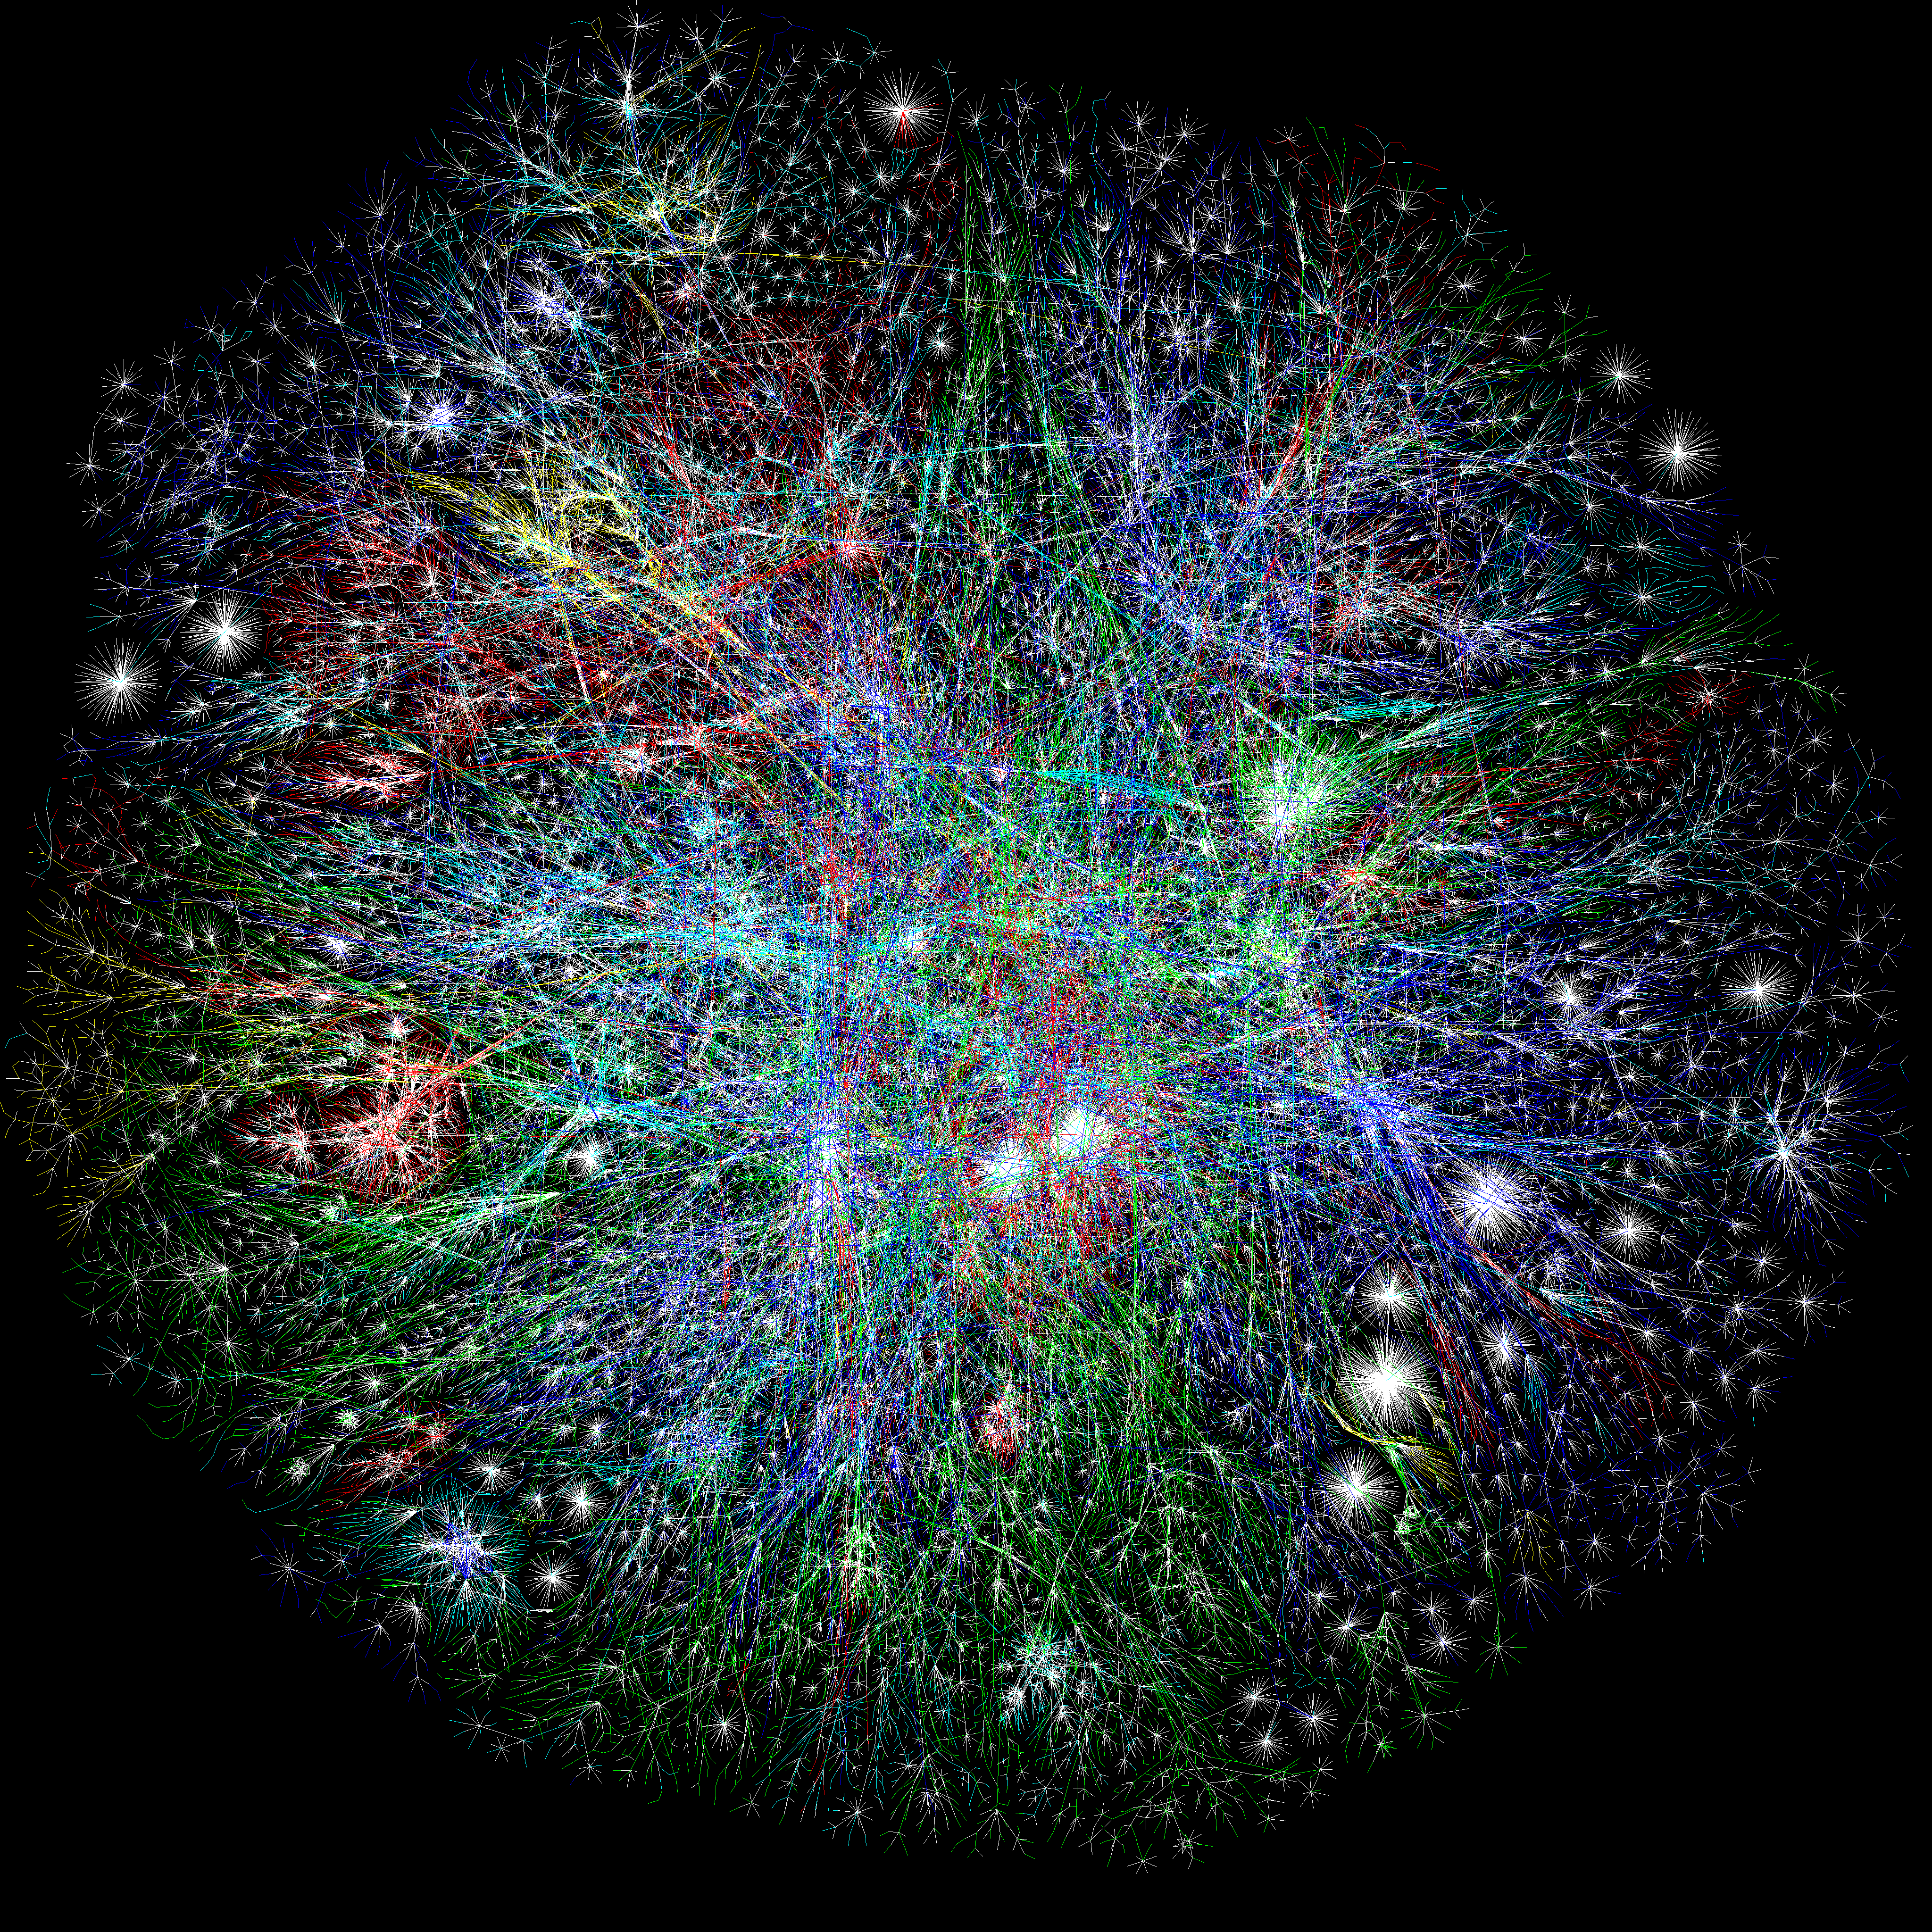
\includegraphics[width=\paperwidth]{media/internet.png}
            };
        
        \pause
        
            \node[anchor=north west,inner sep=0pt] at (0, 0) {
                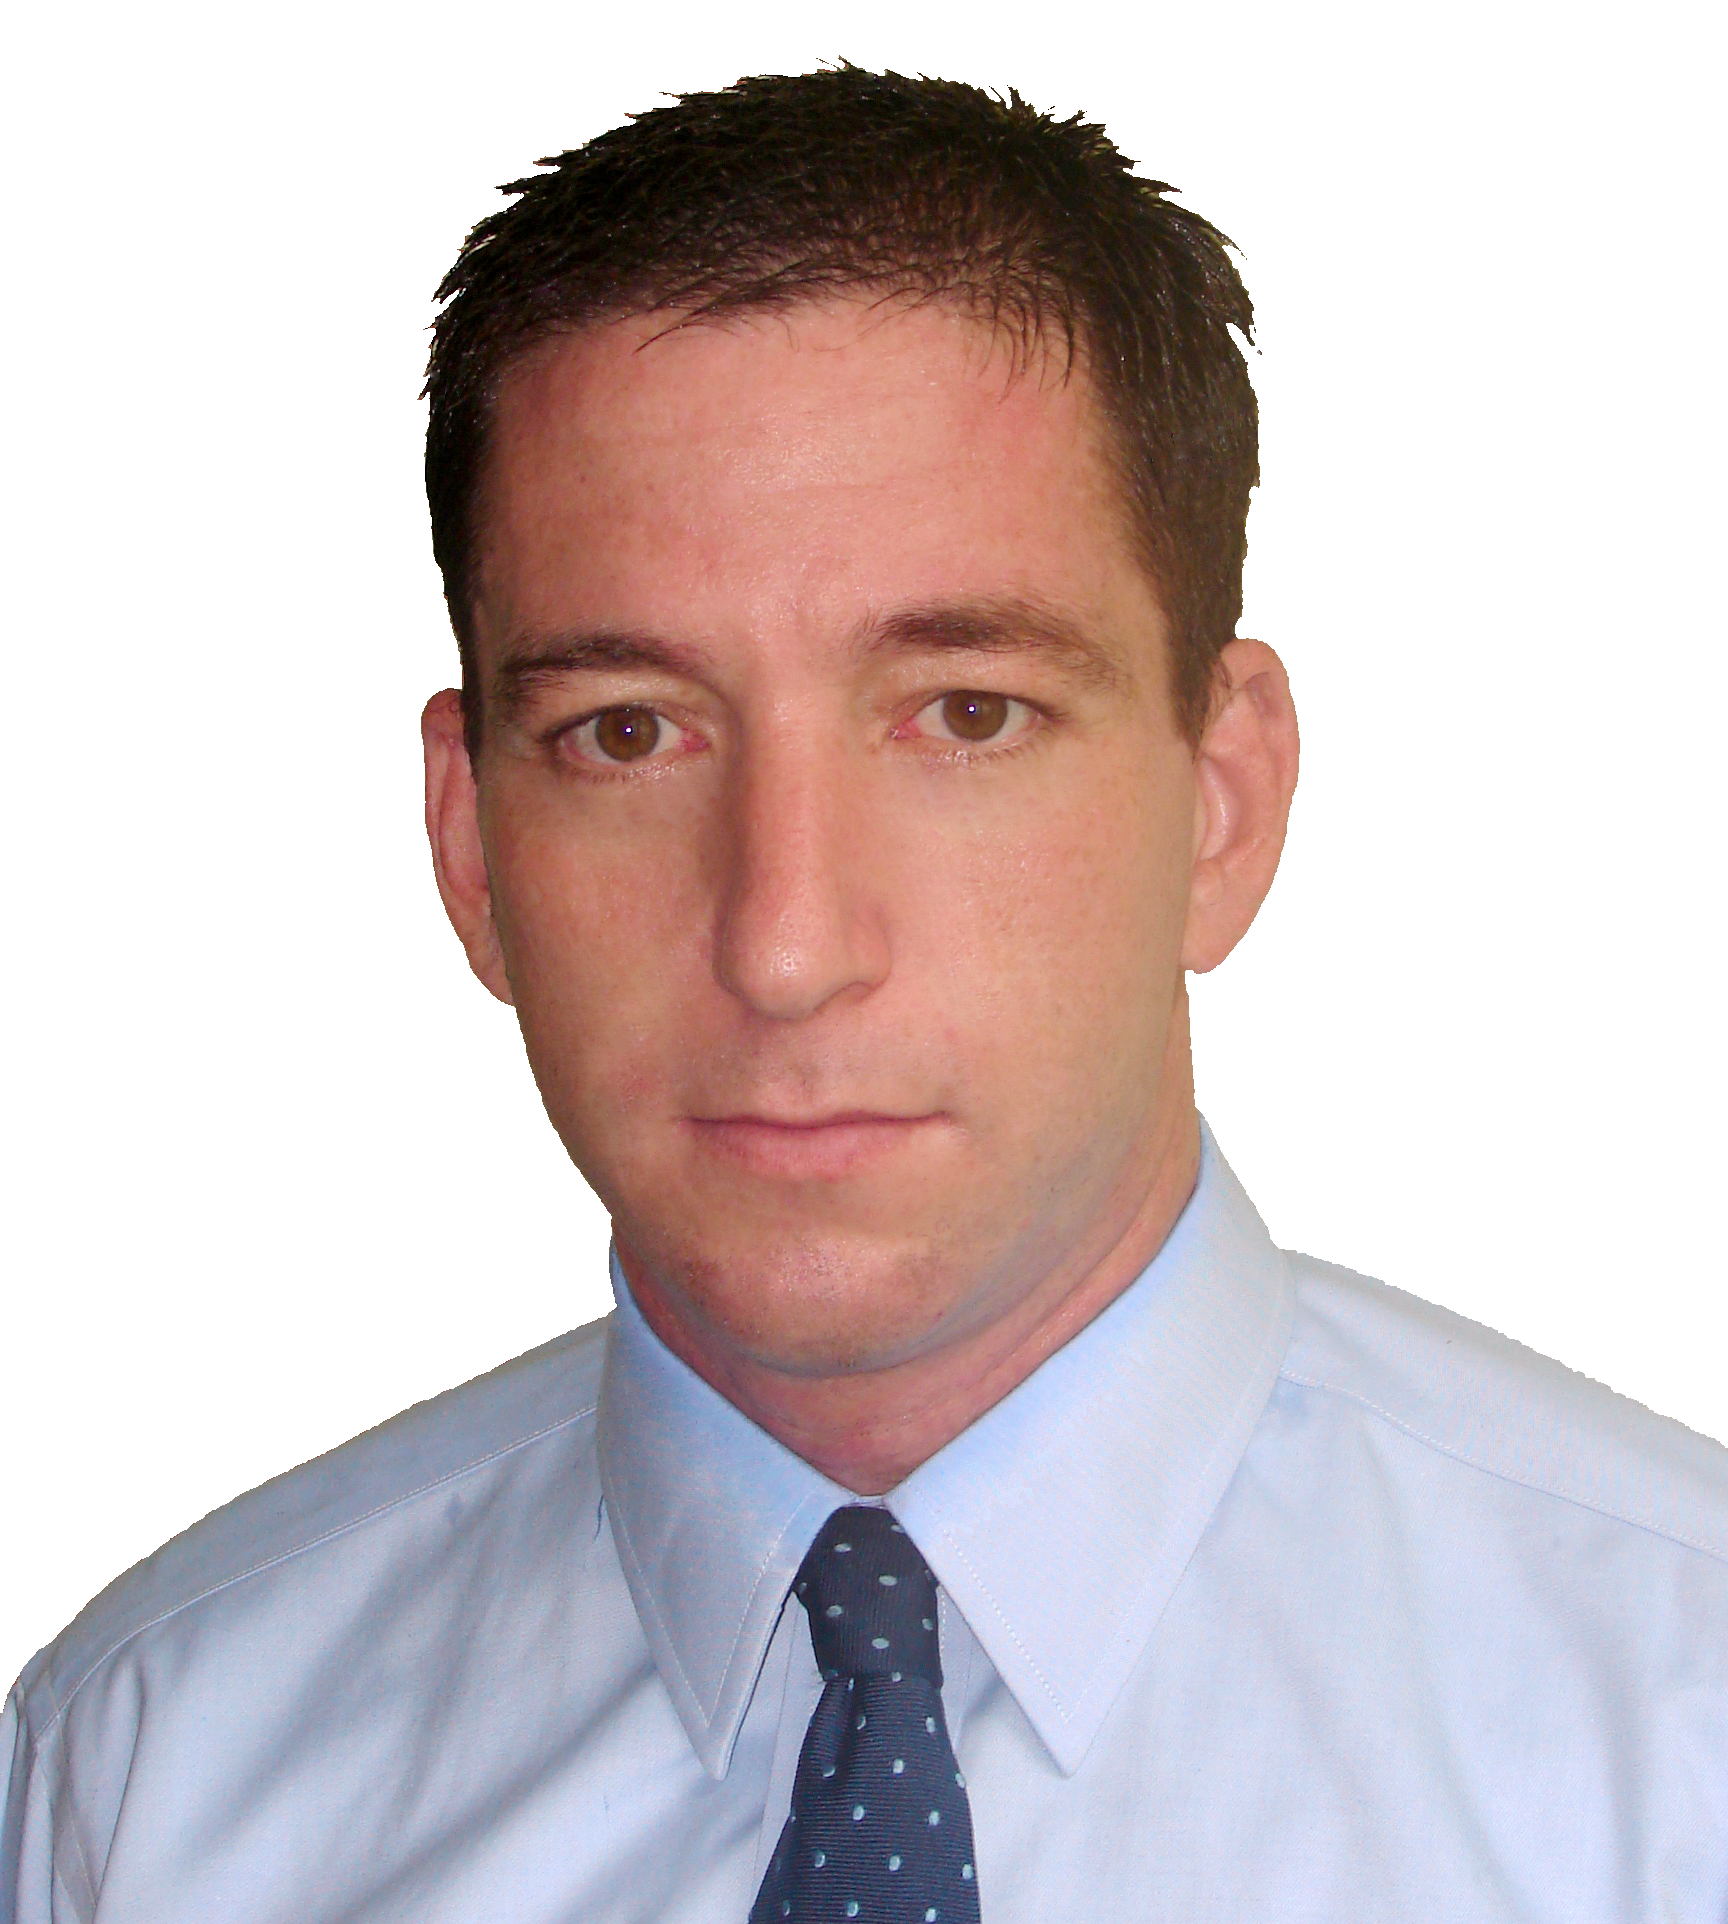
\includegraphics[width=65pt]{media/greenwald.png}
            };
        
            \node[anchor=north west,inner sep=0pt] at (0, -4) {
                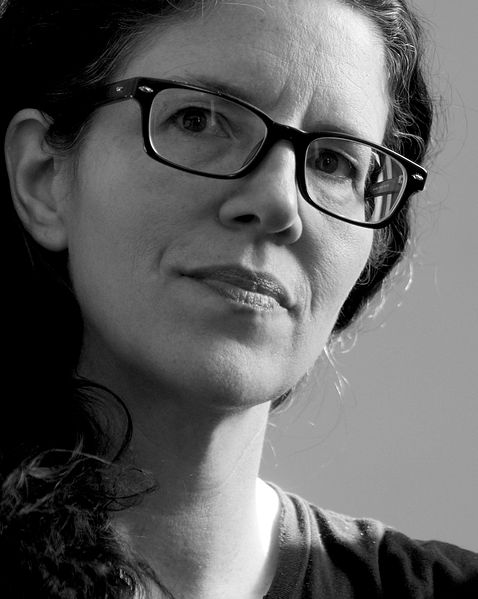
\includegraphics[width=65pt]{media/poitras.jpg}
            };
       
            \node[anchor=north west,inner sep=0pt] at (8, -5) {
                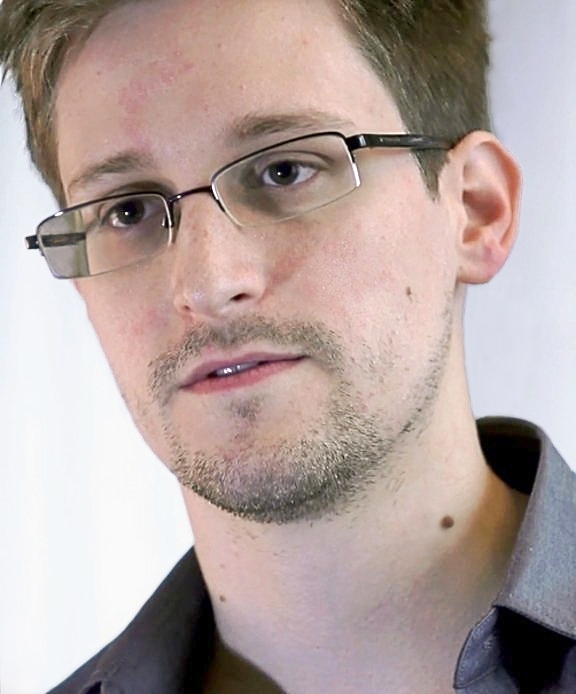
\includegraphics[width=65pt]{media/snowden.jpg}
            };

        \pause
        
            \node[anchor=north west,inner sep=0pt] at (8, 1) {
                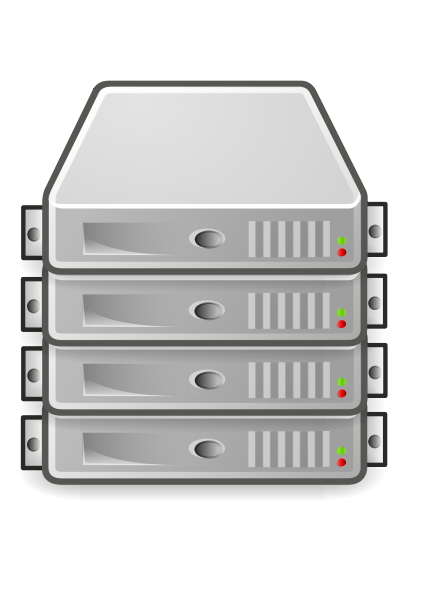
\includegraphics[width=60pt]{media/servers.png}
            };
        	 \draw [<->, line width=0.2cm, red, dashed] (9, -5) -- (9, -1.5); % line from server to snowden
        	 
        % \pause
        	 
        	 \draw [<->, line width=0.2cm, red, dashed] (2.5, -2) -- (8, 0); % line from server to greenwald
        	 \draw [<->, line width=0.2cm, red, dashed] (2.5, -6) -- (8, -1.5); % line from server to poitras
        	 
        	 \node[anchor=north west,inner sep=0pt] at (9, -3) {
                
\includegraphics[width=30pt]{media/lock.png}
            };
            \node[anchor=north west,inner sep=0pt] at (4, -4) {
                
\includegraphics[width=30pt]{media/lock.png}
            };

			\pause            
            
            \node[anchor=north west,inner sep=0pt] at (4, -0.5) {
                
\includegraphics[width=30pt]{media/attack.png}
            };
            
             \node[anchor=north west,inner sep=0pt] at (9, 0) {
                
\includegraphics[width=30pt]{media/attack.png}
            };
        	 
        \end{tikzpicture}
        
         \note {
     		Take the internet as an example. \\
			Well, lets say we have two persons who have good reasons \\
			to communicate confidentiality over such a network.		\\
			\ldots \\
			Laura POITRAS, glenn greenwald \\
			and of course edward snowden
			\ldots \\
			
			 \textbf{provided SSL / TLS is secure}
     }
     \end{frame}    
}

%%%%%%%%%%%%%%%%%%%%%%%%%%%%%%%%%%%%%%%%%%%%%%%%%%%%%%%%%%%%%%%%%%%%%%%%%%%%

\begin{frame}
	\frametitle{Other Examples}
	
	\begin{itemize}
		\item Health Details
		\item Company Secrets
		\item Journalism
		\item Activism
	\end{itemize}

\end{frame}

%%%%%%%%%%%%%%%%%%%%%%%%%%%%%%%%%%%%%%%%%%%%%%%%%%%%%%%%%%%%%%%%%%%%%%%%%%%%

\begin{frame}
	\frametitle{Problem Statement}

	\begin{itemize}
		\item Message Confidentiality
		\item Message Integrity
		\item Sender Authentication
		\item Anonymity?
	\end{itemize}

\end{frame}

%%%%%%%%%%%%%%%%%%%%%%%%%%%%%%%%%%%%%%%%%%%%%%%%%%%%%%%%%%%%%%%%%%%%%%%%%%%%
\section{openPGP}
\sectionheader{openPGP}
%%%%%%%%%%%%%%%%%%%%%%%%%%%%%%%%%%%%%%%%%%%%%%%%%%%%%%%%%%%%%%%%%%%%%%%%%%%%


\begin{frame}
	\frametitle{PGP History}

	\begin{itemize}
		\item Pretty Good Privacy
		\item 1991: PGP created by Phil Zimmermann 
		\item \textit{most widely used email encryption software} \cite{zimmermann}
		\item 1998: PGP 5 standardized: \textbf{OpenPGP (RFC 4880)}
		\item 2010: PGP assets sold to Symantec \\ for \$ 300.000.000 (Enterprise Security)
	\end{itemize}
	
	\note{
		 Zimmermann: anti-nuclear activist \\
		 PGP: invented to store message on message boards	
	}

\end{frame}

%%%%%%%%%%%%%%%%%%%%%%%%%%%%%%%%%%%%%%%%%%%%%%%%%%%%%%%%%%%%%%%%%%%%%%%%%%%%

% explain what gpg is, what pgp is, what openpgp is and what jog is (bouncycastle, too)

\begin{frame}

	\begin{itemize}
		\item Standard: openPGP (RFC 4880 et al.)
		\item Implementations:
		\begin{itemize}
			\item PGP (Zimmermann, Symantec)
			\item GnuPG / GPG (GNU)
			\item APG (Android)
			\item End-to-End (Google Chrome)
			\item Bouncycastle (Java)
			\item \textit{Java Privacy Guard} (IAIK-JCE)
		\end{itemize}
	\end{itemize}

\end{frame}

%%%%%%%%%%%%%%%%%%%%%%%%%%%%%%%%%%%%%%%%%%%%%%%%%%%%%%%%%%%%%%%%%%%%%%%%%%%%

\begin{frame}
	\frametitle{openPGP}
	
	\begin{itemize}
		\item Combines Symmetric-Key Cryptography \\and Public-Key Cryptography
		\item + Hashing
		\item + Data Compression
		\item + Trust Model 
	\end{itemize}
	
\end{frame}


%%%%%%%%%%%%%%%%%%%%%%%%%%%%%%%%%%%%%%%%%%%%%%%%%%%%%%%%%%%%%%%%%%%%%%%%%%%%

\begin{frame}

	\frametitle{De-/Encryption}

% how does pgp do that? -> explain message signing (integrity)

	\begin{itemize}
		\item Encrypt Data Symmetric, only Symmetric-Key with Public-Key
		\item Multiple Receiver: Encrypt Data Oonly once \\
		\item Symmetric Cipher: IDEA, 3DES, AES, CAST5, \ldots 
		\item Public-Key Cipher: RSA, ElGamal \\
				\small Keysize $\geq 2048 bits$ \cite{nist} 
	\end{itemize}

\end{frame}

%%%%%%%%%%%%%%%%%%%%%%%%%%%%%%%%%%%%%%%%%%%%%%%%%%%%%%%%%%%%%%%%%%%%%%%%%%%%

\begin{frame}

%\frametitle{openPGP: De-/Encryption}

% how does pgp do that? -> explain encryption (confidentiality)

	\begin{tikzpicture}[remember picture,overlay]
		\only<1-4> \node[anchor=south west,inner sep=0pt] at (-1.5, -7) {
			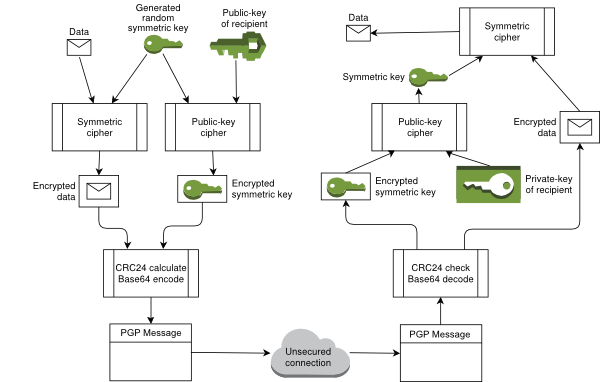
\includegraphics[width=1.2\textwidth]{media/pgp.png}
		};
		
		%\pause
		
		\only<-1> \draw [fill=white, white] (-1.5, -3.25) rectangle (5,-0.95);
		
		%\pause
		
		\only<-2> \draw [fill=white, white] (-1.5, -3.25) rectangle (5,-7);
		\only<-2> \draw [fill=white, white] (5, -5.5) rectangle (13,-7);

		%\pause		
		
		\only<-3> \draw [fill=white, white] (5, 2) rectangle (13,-5.7);
			
     \end{tikzpicture}		

\end{frame}

%%%%%%%%%%%%%%%%%%%%%%%%%%%%%%%%%%%%%%%%%%%%%%%%%%%%%%%%%%%%%%%%%%%%%%%%%%%%

\begin{frame}

	\frametitle{Digital Signatures}

% how does pgp do that? -> explain message signing (integrity)

	\begin{itemize}
		\item Hash Message Body \&{} Sign Hash with Private Key
		\item Sign Other Keys ($\rightarrow$ Trust Model)	 \\
		\item Hash Algorithms: MD5, SHA-1 SHA-2, RIPE-MD
		\item Signature Cipher: RSA, DSA \\
			\small Keysize $\geq 112 bits$ \cite{nist} 
	\end{itemize}

\end{frame}

%%%%%%%%%%%%%%%%%%%%%%%%%%%%%%%%%%%%%%%%%%%%%%%%%%%%%%%%%%%%%%%%%%%%%%%%%%%%

\sectionheader{So \ldots PGP == S/MIME ?}

%%%%%%%%%%%%%%%%%%%%%%%%%%%%%%%%%%%%%%%%%%%%%%%%%%%%%%%%%%%%%%%%%%%%%%%%%%%%

\begin{frame}

% NO! => explain authentizy => web of trust
% advantages: does not need ca, everyone is ca
% dissadvantages: social graph public (again: no anonymity!), how secure is a ca? usability?
% concusio: bussines vs private? central vs decentral

	\frametitle{Web Of Trust}

	\begin{itemize}
		\item Decentralized Trust Model \\ (Can be centralized)
		\item No Certificate Authority
	\end{itemize}	
	
	\begin{itemize}
	  % \item Keyserver Statistics: \url{sks-keyservers.net/status}
		\item Pathfinder:          \url{pgp.cs.uu.nl/doc/faq.html}
		\item Key-Set Analysis: \url{pgp.cs.uu.nl/plot}
	\end{itemize}

\end{frame}

%%%%%%%%%%%%%%%%%%%%%%%%%%%%%%%%%%%%%%%%%%%%%%%%%%%%%%%%%%%%%%%%%%%%%%%%%%%%

\begin{frame}
	\frametitle{Revisiting Problem Statement}

	\begin{itemize}
		\item Message Confidentiality: \textbf{Encryption} 
		\item Message Integrity:          \textbf{Digital Signatures} 
		\item Sender Authentication:    	\textbf{Web Of Trust}
		\item Anonymity? Tor, I2P, \ldots
	\end{itemize}

	\note{
		Metadata-less PGP Encryption is possible	
	}

\end{frame}

%%%%%%%%%%%%%%%%%%%%%%%%%%%%%%%%%%%%%%%%%%%%%%%%%%%%%%%%%%%%%%%%%%%%%%%%%%%%
\section{Java Privacy Guard}
%%%%%%%%%%%%%%%%%%%%%%%%%%%%%%%%%%%%%%%%%%%%%%%%%%%%%%%%%%%%%%%%%%%%%%%%%%%%

\begin{frame}[fragile]
	\frametitle{Quelltexte}
	\begin{spacing}{1}
	\begin{semiverbatim}
SUCHE (A,x)
1: i = 0
2: WHILE i<n
3:     i = i+1
4:     \alert{IF A[i]=x THEN RETURN i}
5: ELSE RETURN -1
	\end{semiverbatim}
	\end{spacing}
\end{frame}

%%%%%%%%%%%%%%%%%%%%%%%%%%%%%%%%%%%%%%%%%%%%%%%%%%%%%%%%%%%%%%%%%%%%%%%%%%%%


\begin{frame}
	\frametitle{Zwei Inhalte Links/Rechts\\Wahlweise Text/Grafik}
	\begin{columns}[onlytextwidth]
		\begin{column}{0.5\textwidth}
			\begin{itemize}
				\item Lorem ipsum dolor sit amet, consectetur 
				\item adipisicing elit, sed do eiusmod tempor 
				\item incididunt ut labore et dolore magna aliqua. 
				\item Ut enim ad minim veniam, quis nostrud 
			\end{itemize}
		\end{column}
		\begin{column}{0.5\textwidth}
			\begin{center}
			
\includegraphics[width=0.5\textwidth]{logo.pdf}\\
			Grafik in Spalte 2
			\end{center}
		\end{column}
	\end{columns}
\end{frame}



\begin{frame}
	\frametitle{Nur Titel \\maximal 2-zeilig}
\end{frame}



%%%%%%%%%%%%%%%%%%%%%%%%%%%%%%%%%%%%%%%%%%%%%%%%%%%%%%%%%%%%%%%%%%%%%%%%%%%%
\section{Summary \&{} Outlook}
%%%%%%%%%%%%%%%%%%%%%%%%%%%%%%%%%%%%%%%%%%%%%%%%%%%%%%%%%%%%%%%%%%%%%%%%%%%%

\begin{frame}
	\frametitle{Summary}
	
	\begin{itemize}
		\item Studied RFC 4880
		\item Studied IAIK-JCE
		\item Implemented:
		\begin{itemize}
			\item Reading ASCII-Armor (Base 64 + CRC24)
			\item Parsing PGP Message Objects (\textit{Packets})
			\item Key Management (Simple Keychain)
			\item Message Decryption (RSA \&{} ElGamal)
			\item Signature Validation (RSA \&{} DSA)
			\item Decompression
		\end{itemize}
	\end{itemize}
	
\end{frame}

%%%%%%%%%%%%%%%%%%%%%%%%%%%%%%%%%%%%%%%%%%%%%%%%%%%%%%%%%%%%%%%%%%%%%%%%%%%%

\begin{frame}
	\frametitle{Future (Research) Outlook}
	
	\begin{itemize}
		%\item Master Project
		\item Message Encryption and Signature Validation
		\item Missing parts of RFC 4880 (Partial body length, \ldots)
		\item RFC 6637: ECC
		\item Keyservers?
	\end{itemize}
	Out of scope:
	\begin{itemize}
	    \item RFC 3156: PGP/MIME
		\item Provide Anonymity? (Metadata!)%\footnotemark
		\item Provide Integrity for Mail-Headers?
		\item Protocol/Implementation Usability?
	\end{itemize}
	%\footnotetext{http://grimoire.ca/gpg/terrible}
	
	\note{
		 Master Project, Summer job, \\
		 further research?	
	}
\end{frame}

%%%%%%%%%%%%%%%%%%%%%%%%%%%%%%%%%%%%%%%%%%%%%%%%%%%%%%%%%%%%%%%%%%%%%%%%%%%%

\sectionheader[Questions? Remarks?]{Thank You for Your Attention}

%%%%%%%%%%%%%%%%%%%%%%%%%%%%%%%%%%%%%%%%%%%%%%%%%%%%%%%%%%%%%%%%%%%%%%%%%%%%
  
\begin{frame}
\frametitle{Sources}

\begin{thebibliography}{1}
\scriptsize

	\bibitem{snowden} Laura Poitras \url{https://commons.wikimedia.org/wiki/File:Edward_Snowden-2.jpg} 
	
	\bibitem{greenwald} Glenn Greenwald  \url{https://en.wikipedia.org/wiki/File:Glenn_greenwald_portrait_transparent.png}
	
	\bibitem{poitras} Katy Scoggin \url{https://commons.wikimedia.org/wiki/File:Laura_Poitras_2014.jpg}
	
	\bibitem{servers} Regionales RechenZentrum Erlangen  \url{https://commons.wikimedia.org/wiki/Category:RRZE-Icon-Set}
	
	\bibitem{internet}  The Opte Project \url{http://www.opte.org/the-internet}
	
	\bibitem{zimmermann} \url{http://www.philzimmermann.com/EN/background/index.html}
	
	\bibitem{nist} Recommendation for Key Management, Special Publication 800-57 Part 1 Rev. 3, NIST, 07/2012. \url{http://www.keylength.com/en/4/}

\end{thebibliography}
\end{frame}


\end{document}
%%%%%%%%%%%%%%%%%%%%%%%%%%%%%%%%%%%%%%%%%%%%%%%%%%%%%%%%%%%%%%%%%%%%%%%%%%%%

%% EOF
